\documentclass{article}

% Language setting
% Replace `english' with e.g. `spanish' to change the document language
\usepackage[english]{babel}

% Set page size and margins
% Replace `letterpaper' with `a4paper' for UK/EU standard size
\usepackage[letterpaper,top=2cm,bottom=2cm,left=3cm,right=3cm,marginparwidth=1.75cm]{geometry}

% Useful packages
\usepackage{amsmath}
\usepackage{float}
\usepackage{graphicx}
\usepackage[colorlinks=true, allcolors=blue]{hyperref}

\title{Računalniška grafika zapiski}
\author{Tim Hajdinjak}

\begin{document}
\maketitle

\section{Matematične osnove}

Osnovni pojmi, brez katerih žal ne gre

\begin{itemize}
\item stolpčna matrika: $\begin{bmatrix} 2,9 \\ -4,6 \\ 0 \end{bmatrix}$
\item vrstična matrika:  $\begin{bmatrix} 12,5 & -9,32 & 0 \end{bmatrix}$
\item transponiranje: pomeni zamenjavo osi dveh matrik: $\begin{bmatrix} 1,3 & -4,1 & 0,0 \end{bmatrix}^T = \begin{bmatrix} 1,3 \\ -4,1 \\ 0,0 \end{bmatrix}$
\item enakost matrik: dve matriki sta si enaki, če imata enako število elementov po obeh oseh, in so vsi vsebovani elementi na enakih mestih
\item vektor: predstavljen kot matrika, pomeni premik iz točke v točko in vektorji nimajo lokacije
\item seštevanje matrik: $a + b = c \iff c_i = a_i + b_i$, intuitivno: 
\begin{figure}[H]
\centering
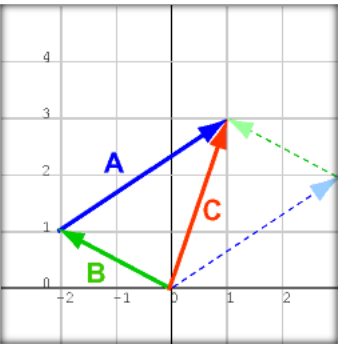
\includegraphics[width=25mm]{src/sestevanje_vektorjev.png}
\caption{Geometrijsko sestevanje vektorjev. (iz repa vektorja 1 na glavo vektorja 2)}
\end{figure}
\item enota za seštevanje: $a + 0 = 0 + a = a \iff \begin{bmatrix} 3 & -1 \end{bmatrix} + \begin{bmatrix} 0 & 0 \end{bmatrix} = \begin{bmatrix} 3 & -1 \end{bmatrix}$
\item odštevanje matrik: $a - b = c \iff c_i = a_i - b_i$
\item množenje s skalarjem: $\alpha * a = b \iff b_i = \alpha * a_i$
\item inverz za seštevanje: $a - a = a + -a = a + (-1)a=0 \iff \begin{bmatrix} 2 & 5 \end{bmatrix} - \begin{bmatrix} 2 & 5 \end{bmatrix} = \begin{bmatrix} 2 & 5 \end{bmatrix} + \begin{bmatrix} -2 & -5 \end{bmatrix}=\begin{bmatrix} 0 & 0 \end{bmatrix}$
\item NORMA oz. dolžina vektorja: $h = \begin{bmatrix} x \\ y \end{bmatrix} \Longrightarrow \lVert h \rVert = \sqrt{x^2 + y^2}, oz. \lVert a \rVert = \sqrt{\sum_{i=1}^n a_i^2}$ (L2 norm oz. evklidska razdalja). Splošna norma: $\lVert a \rVert_p = \sqrt[p]{\sum_{i=1}^n |a_i|^p}$. Torej, če na izpitu reče druga splošna norma, namesto p pišeš 2. Neskončna norma $\to$ dolžina se bliža maksimalni vrednosti vektorja. 
\item enotski vektor, pomeni vektor dolžine 1, $\lVert e \rVert = 1$
\item normalizacija: $v = \begin{bmatrix} v_x \\ v_y \\ v_z \end{bmatrix} \Longrightarrow \hat{v} = v / \lVert v \rVert = \begin{bmatrix} v_x/\lVert v \rVert \\ v_y/\lVert v \rVert \\ v_z/\lVert v \rVert \end{bmatrix}, \hat{v} = $ enotskost vektorja 
\item skalarni produkt: $u = \begin{bmatrix} u_0 \\ u_1 \\ u_2 \end{bmatrix}, v = \begin{bmatrix} v_0 \\ v_1 \\ v_2 \end{bmatrix} \Longrightarrow u * v = u_0*v_0 + u_1*v_1 + u_2*v_2$. Pravimo mu tudi "detektor pravokotnosti", saj:
\begin{enumerate}
    \item $u*v = 0 \to$ vektorja pravokotna
    \item $u*v < 0 \to$ iztegnjen kot
    \item $u*v > 0 \to$ ostri kot
    \item $\hat{a} * \hat{b} \to$ vrednosti med $[-1, 1],-1 = 180^\circ, 0 = 90^\circ, 1 = 0^\circ$
\begin{figure}[H]
\centering
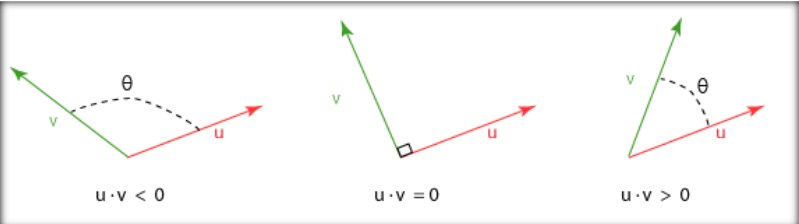
\includegraphics[width=100mm]{src/ortogonalnost.png}
\caption{2 vektorja sta ortogonalna, če je skalarni produkt enak 0 (oz. sta si pravokotna)}
\end{figure}
\begin{figure}[H]
\centering
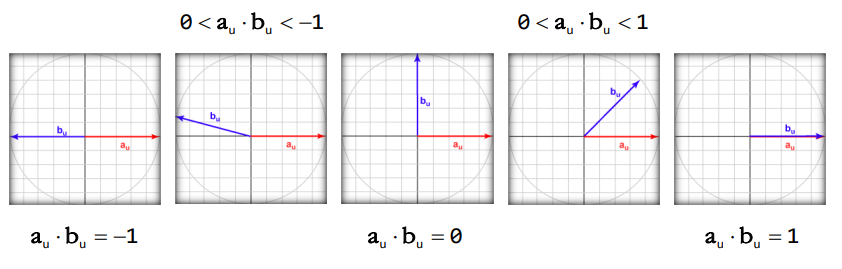
\includegraphics[width=100mm]{src/skalarni_produkt_enotskih_vektorjev.png}
\caption{Skalarni produkt enotskih vektorjev}
\end{figure}
\end{enumerate}
Še par pravil oz. posebnosti pri skalarnih produktih:
\begin{itemize}
    \item $u * v = \lVert u \rVert * \lVert v \rVert * \cos{\alpha}$
    \item $v * v = \lVert v  \rVert^2$, norma
    \item $u * 0 = 0 * u = 0$, skalarni produkt z vektorjem 0
    \item $0 * 0 = 0$, skalarni produkt vektorja 0
    \item $u * v = v * u$, komutativnost
    \item $u * (v+w) = u*v + u*w$, distributivnost za seštevanje
    \item $(\alpha u)*v = u * (\alpha v) = \alpha * (u * v)$, homogenost za množenje s skalarjem
    \item $u \perp v \iff u * v = 0$, skalarni produkt ortogonalnih (pravokotnih) vektorjev
    \item asociativnost: nedefinirana operacija
\end{itemize}
\item linearna neodvisnot, projekcija vektorja na vektor: $kv = \lVert w \rVert (w_u * v_u)*v_u$
\begin{figure}[H]
\centering
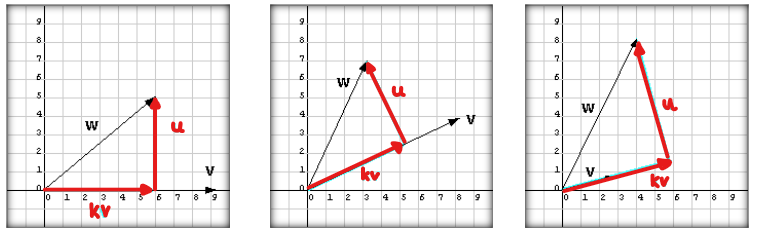
\includegraphics[width=100mm]{src/projekcija_vektorja_na_vektor.png}
\caption{Projekcija vektorja na vektor}
\end{figure}
Postopek pri linearne neodvisnost:
\begin{enumerate}
    \item Izračunaj dolžine vektorjev: $\lVert w \rVert = w * w, \lVert v \rVert = v * v$ 
    \item Izračunaj enotske vektorje: $w_u = w/ \lVert w \rVert, v_u = v/ \lVert v \rVert$
    \item Izračunaj kosinus kota med vektorji: $\cos{\alpha} = w_u * v_u$
    \item Združi v projekcijo: $kv = \lVert w \rVert (w_u * v_u)*v_u$
    \item Izračunaj ortogonalni vektor: $u = w - kv$
\end{enumerate}
\item Vektorski produkt: $u = \begin{bmatrix} u_x \\ u_y \\ u_z \end{bmatrix}, v = \begin{bmatrix} v_x \\ v_y \\ v_z \end{bmatrix}, u \times v = \begin{bmatrix} u_yv_z - u_zv_y \\ u_zv_x - u_xv_z \\ u_xv_y - u_yv_x \end{bmatrix}$
\begin{figure}[H]
\centering
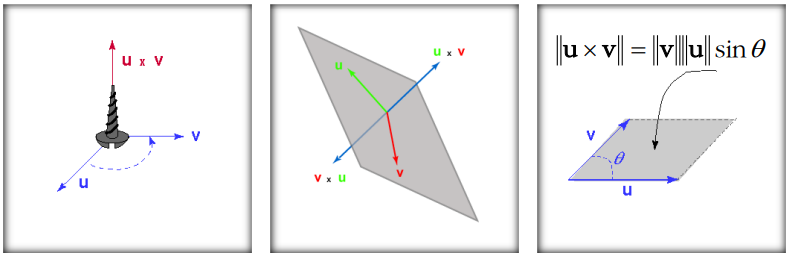
\includegraphics[width=100mm]{src/vektorski_produkt.png}
\caption{Vektorski produkt intuitivno}
\end{figure}
\begin{figure}[H]
\centering
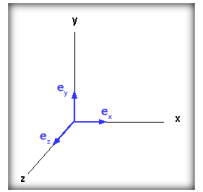
\includegraphics[width=30mm]{src/enotski_vektorji.png}
\caption{Enotski vektorji, ki tvorijo prostor $R^3$, imajo normo (dolžino) 1 in so vzajemno pravokotni. Pri tem je $e_x = (1,0,0), e_y = (0,1,0), e_z = (0,0,1)$}
\end{figure}
Zakonitosti pri vektorskem produktu:
\begin{enumerate}
    \item $u \times v = -(v \times u)$, antikomutativnost
    \item $u \times (v + w) = u \times v + u \times w$, distributivnost za seštevanje
    \item $(\alpha u) \times v = u \times (\alpha v) = \alpha(u \times v)$, homogenost za množenje s skalarjem
    \item Asociativnost ne obstaja:  $u \times (v \times w) \not = (u \times v) \times w$
    \item $u \parallel v \iff u \times v = 0$, vektorski produkt kolinearnih vektorjev
    \item $u \times 0 = 0 \times v = 0$, vektorski produkt vektorja 0
    \item $0 \times 0 = 0$, vektorski produkt z vektorjem 0
    \item $e_x \times e_y = e_z, e_y \times e_z = e_x, e_z \times e_x = e_y$, vektorski produkt koordinatnih osi, zanimivost: vidimo lahko desno pravilo
\end{enumerate}
\item Splošna matrika, notacija: $A_{m \times n} = \begin{bmatrix}
    a_{11} & a_{12} & \cdots & a_{1n} \\
    a_{21} & a_{22} & \cdots & a_{2n} \\
    \vdots & \vdots & \ddots & \vdots \\
    a_{m1} & a_{m2} & \cdots & a_{mn}
\end{bmatrix}$
\item Seštevanje matrik: $A + B = C \iff c_{ij} = a_{ij} + b_{ij}$, primer: $\begin{bmatrix} 2 & 0 \\ -1 & 2 \\ 3 & 5 \end{bmatrix} + \begin{bmatrix} 
 1 & 3 \\ -1 & 2 \\2 & -1 \end{bmatrix} = \begin{bmatrix} 3 & 3 \\ -2 & 4 \\ 5 & 4 \end{bmatrix}$
 Zakonitosti pri seštevanju splošnih matrik:
 \begin{enumerate}
     \item Možno le, če sta matriki enakih dimenzij! 
     \item $A + B = B + A$, komutativnost
     \item $(A + B) + C = A + (B + C)$, asociativnost
     \item $A + 0 = 0 + A = A$, enota za seštevanje
     \item $A - A = A + (-1)A = 0$, inverz za seštevanje
 \end{enumerate}
\item Množenje matrik s skalarjem: $\alpha A = B \iff b_{ij} = \alpha a_{ij}$, primer: $3 * \begin{bmatrix} 2 & 0 \\ -1 & 2 \\ 3 & 5 \end{bmatrix} = \begin{bmatrix} 6 & 0 \\ -3 & 6 \\ 9 & 15 \end{bmatrix}$
Zakonitosti pri množenju matrik s skalarjem:
\begin{enumerate}
    \item $\alpha (A + B) = \alpha A + \alpha B$, distributivnost seštevanja matrik
    \item $(\alpha + \beta)A = \alpha A + \beta A$, distributivnost seštevanja skalarjev
    \item $(\alpha \beta)A = \alpha (\beta A)$, asociativnost
    \item $(-1)A = -A$, množenje s skalarjem -1
\end{enumerate}
\item Množenje matrik: $A_{n \times m}B_{m \times p} = C_{n \times p} \iff c_{ij} = \sum_{k=1}^m a_{ik}b_{kj}$
\begin{figure}[H]
\centering
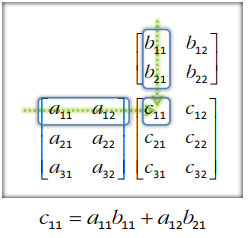
\includegraphics[width=40mm]{src/mnozenje_matrik.png}
\caption{Miselni vzorec za množenje splošnih matrik}
\end{figure}
Zakonitosti pri množenju matrik:
\begin{enumerate}
    \item $AB \not = BA$, komutativnost ne velja
    \item $(AB)C = A(BC)$, asociativnost
    \item $A(B + C) = AB + AC$, distributivnost za seštevanje
    \item $(A + B)C = AC + BC$, distributivnost za seštevanje
    \item $(\alpha A)B = A(\alpha B) = \alpha (AB)$, homogenost za množenje s skalarjem
    \item $0A = 0$, množenje s skalarjem 0
    \item $A0 = 0A = 0$, množenje z matriko 0
\end{enumerate}
\item Enota za množenje oz. identiteta: $I_n = \begin{bmatrix} 
1 & 0 & 0 & \cdots & 0 \\ 0 & 1 & 0 & \cdots & 0 \\ 0 & 0 & 1 & \cdots & 0 \\ \vdots & \vdots & \vdots & \ddots & \vdots \\ 0 & 0 & 0 & \cdots & 1 \end{bmatrix}_{n \times n}$, 1 po diagonali
\begin{enumerate}
    \item $AB = BA = I \iff B = A^{-1}$
    \item $(ABC)^{-1} = C^{-1}B^{-1}A^{-1}$, inverz za množenje
\end{enumerate}
\item Transponiranje: $A^T = B \iff b_{ij} = a_{ji}$
Lastnosti transponiranja:
\begin{enumerate} 
    \item $(A^T)^T = A$
    \item $(\alpha A)^T = \alpha A^T$
    \item $(A + B)^T = A^T + B^T$
    \item $(ABC)^T = C^TB^TA^T$
    \item $(A^{-1})^T = (A^T)^{-1}$
\end{enumerate}
\end{itemize}

\section{Transformacije in homogene koordinate}

\section{Some examples to get started}

\subsection{How to create Sections and Subsections}

Simply use the section and subsection commands, as in this example document! With Overleaf, all the formatting and numbering is handled automatically according to the template you've chosen. If you're using the Visual Editor, you can also create new section and subsections via the buttons in the editor toolbar.

\subsection{How to include Figures}

First you have to upload the image file from your computer using the upload link in the file-tree menu. Then use the includegraphics command to include it in your document. Use the figure environment and the caption command to add a number and a caption to your figure. See the code for Figure \ref{fig:frog} in this section for an example.

Note that your figure will automatically be placed in the most appropriate place for it, given the surrounding text and taking into account other figures or tables that may be close by. You can find out more about adding images to your documents in this help article on \href{https://www.overleaf.com/learn/how-to/Including_images_on_Overleaf}{including images on Overleaf}.

\subsection{How to add Tables}

Use the table and tabular environments for basic tables --- see Table~\ref{tab:widgets}, for example. For more information, please see this help article on \href{https://www.overleaf.com/learn/latex/tables}{tables}. 

\begin{table}[H]
\centering
\begin{tabular}{l|r}
Item & Quantity \\\hline
Widgets & 42 \\
Gadgets & 13
\end{tabular}
\caption{\label{tab:widgets}An example table.}
\end{table}

\subsection{How to add Comments and Track Changes}

Comments can be added to your project by highlighting some text and clicking ``Add comment'' in the top right of the editor pane. To view existing comments, click on the Review menu in the toolbar above. To reply to a comment, click on the Reply button in the lower right corner of the comment. You can close the Review pane by clicking its name on the toolbar when you're done reviewing for the time being.

Track changes are available on all our \href{https://www.overleaf.com/user/subscription/plans}{premium plans}, and can be toggled on or off using the option at the top of the Review pane. Track changes allow you to keep track of every change made to the document, along with the person making the change. 

\subsection{How to add Lists}

You can make lists with automatic numbering \dots

\begin{enumerate}
\item Like this,
\item and like this.
\end{enumerate}
\dots or bullet points \dots
\begin{itemize}
\item Like this,
\item and like this.
\end{itemize}

\end{document}